%%%%%%%%%%%%%%%%%%%%%%%%%% lecture-5
%\begin{frame}[shrink]
%  \frametitle{lecture-5 主要内容}
%  \framesubtitle{选择结构程序设计}
%  \tableofcontents[hideallsubsections]
%  %\tableofcontents[currentsection,hideallsubsections]
%\end{frame}

\section{选择结构和条件判断}

\begin{frame}{选择结构和条件判断}
\begin{columns}
	\column{0.6\textwidth}
	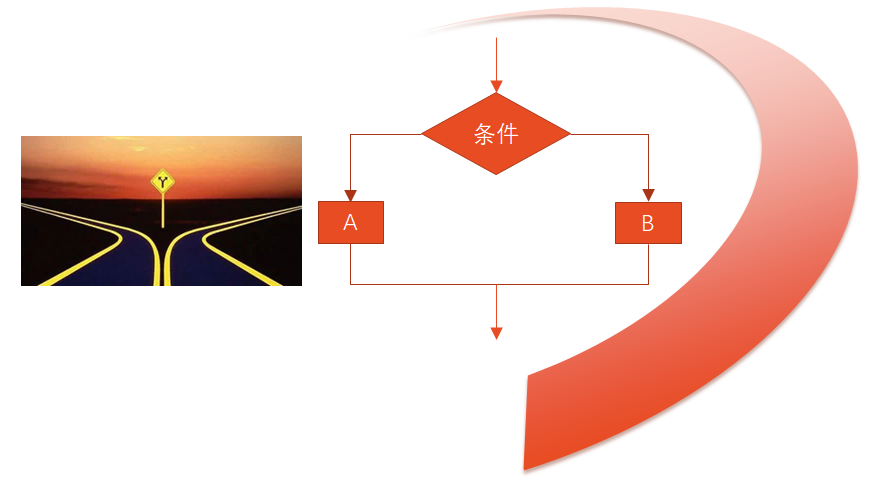
\includegraphics[scale=0.25]{if-case}
	\column{0.4\textwidth}
	\begin{block}{C语言有两种选择语句}
		\begin{itemize}
			\item if语句, 用来实现\textbf{两个分支}的选择结构
			\item switch语句, 用来实现\textbf{多分支}的选择结构
		\end{itemize}
	\end{block}
\end{columns}
\end{frame}

\begin{frame}[fragile]{if(条件表达式)\{ 表达式为真(非0)时执行语句; \}}
\begin{lstlisting}
#include<stdio.h>            // standard input/output编译预处理指令
int main()                   // 主函数
{                            // 函数开始标志
   int a=10;    // 定义变量a为整型数值, 定义变量时,可以指定变量的初值
   if(a>=10)
   {
      printf("a>=10\n"); // \n为换行符
   }
   else
   {
      printf("a<10\n"); // \n为换行符
   }
   return 0;                 // 函数执行完毕返回函数值0
}                            // 函数结束标志
\end{lstlisting}
\end{frame}

\begin{frame}[shrink,fragile]
\small [例4.1 p84] 求$ax^2+bx+c=0$方程的根。$a,b,c$由键盘输入。
\begin{lstlisting}
#include<stdio.h>
#include<math.h>   // 数学库函数        
int main()                   
{  
   double a,b,c,x1,x2,delta;
   scanf("%lf%lf%lf",&a,&b,&c);
   if(b*b-4*a*c < 0) 
   { printf("This equation hasn\'t real roots!\n"); }
   else
   {
      delta = sqrt(b*b-4*a*c);
      x1 = (-b + delta)/(2*a);  x2 = (-b - delta)/(2*a);
      printf("x1=%.2lf,x2=%.2lf\n",x1,x2);
   }
   return 0;           
}                            
\end{lstlisting}
\end{frame}

\begin{frame}[shrink,fragile]
\small [例4.2 p85] 输入两个实数, 按由小到大的顺序输出这两个数。
\begin{columns}
\column{0.45\textwidth}
\begin{lstlisting}
#include<stdio.h>        
int main()                   
{  
   float a,b,t;
   scanf("%f%f",&a,&b); 
   //不好: scanf("%f,%f",&a,&b);
   if(a>b)
   {  //将a和b的值互换
      t=a;
      a=b;
      b=t;
   }
   printf("%.2f,%.2f\n",a,b);
   return 0;           
}
\end{lstlisting} 
\column{0.55\textwidth}
\small
\begin{block}{两个变量值的互换}
a=b;  //把变量b的值赋给变量a,a的值等于b的值\\
b=a;  //再把变量a的值赋给变量b,变量b值没有改变
\end{block}
\textbf{因此, 为了实现互换, 必须借助于第三个变量。}
\end{columns}                           
\end{frame}

\begin{frame}[shrink,fragile]
\small [例4.3 p86] 输入3个数a, b, c, 要求按由小到大的顺序输出。
\begin{lstlisting}
#include<stdio.h>        
int main()                   
{  
    float a,b,c,t;
    scanf("%f%f%f",&a,&b,&c); //不好: scanf("%f,%f,%f",&a,&b,&c);
    if(a>b)
    {
       t=a; a=b; b=t; //借助变量t,实现变量a和变量b互换值
    } //互换后,a小于或等于b     
    if(a>c)
    {
       t=a; a=c; c=t; //借助变量t,实现变量a和变量c互换值
    } //互换后,a小于或等于c       
    if(b>c) //还要
    { 
       t=b; b=c; c=t; //借助变量t,实现变量b和变量c互换值
    }  //互换后,b小于或等于c                       
    printf("%.2f,%.2f,%.2f\n",a,b,c); //顺序输出a,b,c的值
    return 0;  
}
\end{lstlisting}                   
\end{frame}

\section{if语句的一般形式}

\begin{frame}[shrink,fragile]{if(条件表达式)\{ 表达式为真(非0)时执行语句; \}}
\textbf{条件表达式: 关系表达式; 逻辑表达式; 数值表达式。}
\begin{columns}[t]
\column{0.3\textwidth}
\begin{beamerboxesrounded}{形式1(无else)}
\begin{lstlisting}
// 形式1(无else)
if(条件表达式)
{
   多条语句(复合语句);
}
\end{lstlisting}
\end{beamerboxesrounded}
\column{0.3\textwidth}
\begin{beamerboxesrounded}{形式2}
\begin{lstlisting}
// 形式2
if(条件表达式)
{
   多条语句(复合语句);
}
else
{
   多条语句(复合语句);
}
\end{lstlisting} 
\end{beamerboxesrounded}
\column{0.4\textwidth}
\begin{beamerboxesrounded}{形式3(排除式)}
\begin{lstlisting}
// 形式3(排除式)
if(条件表达式1)
{
   多条语句(复合语句);
}
else if(条件表达式2)//可多个
{
   多条语句(复合语句);
}
else
{
   多条语句(复合语句);
}
\end{lstlisting}
\end{beamerboxesrounded}
\end{columns}                        
\end{frame}

\section{关系运算符及其优先次序}

\begin{frame}[shrink,fragile]{关系运算符及其优先次序}
\begin{columns}%[t]
\column{0.5\textwidth}
\begin{lstlisting}
int a=5,b=10,c=20; //以int为例
if(a<b+c) // 相当于a<(b+c)
{ ... }
if(a<=b+c) 
{ ... }
if(a>b+c) 
{ ... }
if(a>=b+c) 
{ ... }
if(a==b+c)//a是否等于(b+c),与a=(b+c)不同
{ ... }
if(a!=b+c) // a不等于(b+c)
{ ... }
\end{lstlisting}
\column{0.5\textwidth}
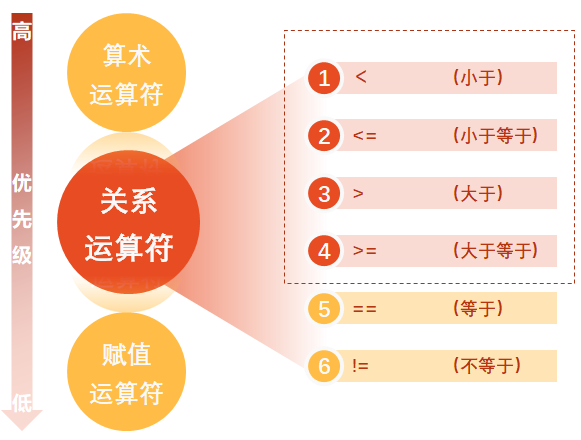
\includegraphics[scale=0.3]{pre}\\
分析:
\begin{lstlisting}
if(a>b==c){...}
if(a=b>c) {...}
\end{lstlisting}
\end{columns}
\end{frame}

\begin{frame}[shrink,fragile]{关系表达式的值, 非0即真}
\begin{block}{关系表达式}
	\small
	\begin{itemize}
		\item 用关系运算符将两个数值或数值表达式连接起来的式子,称为关系表达式。
		\item 关系表达式的值是一个逻辑值,即``真''或``假''。
		\item 在C的逻辑运算中, 以``1''代表``真'',以``0''代表``假''。	
	\end{itemize}
\end{block}
\begin{columns}[T]
\column{0.5\textwidth}
\begin{lstlisting}
int a=3, b=2, c=1, d1, d2; 
d1 = a > b; // d1=1
d2 = a > b > c; //自左至右结合,d2=0
if(d1)
{ printf("执行此语句") }
if(d2) 
{ printf("不执行此语句"); }
\end{lstlisting}
\column{0.5\textwidth}
\begin{lstlisting}
if(d1 = a > b) // d1的值就是表达式的值
{ printf("执行此语句"); }
if(d2 = a > b > c)//d2的值就是表达式的值
{ printf("不执行此语句"); }
\end{lstlisting}
\end{columns}
\end{frame}

\section{逻辑运算符}

\begin{frame}[shrink,fragile]{逻辑运算符}
\begin{lstlisting}
int a=5,b=10,c=0; //以int为例
if(!a) // 逻辑非(NOT), a是非0, 所以!a的值是0
{ ... }
if(a && b) // 逻辑与(AND), a,b均为非0, 所以(a && b)的值为1
{ ... }
if(a || c) // 逻辑或(OR), a,c之一是非0, 即为真
{ ... }
\end{lstlisting}
\end{frame}

\begin{frame}[shrink,fragile]{逻辑运算符真值表}
\centering
\begin{tabular}{|c|c||c|c|c|c|}
\hline 
a       & b      & !a    & !b    & a\&\&b & a||b \\ 
\hline 
真(非0) & 真(非0) & 假(0) & 假(0) & 真(1)  & 真(1) \\ 
\hline
真(非0) & 假(0)   & 假(0) & 真(1) & 假(0)  & 真(1) \\ 
\hline 
假(0)   & 真(非0) & 真(1) & 假(0) & 假(0)  & 真(1) \\ 
\hline 
假(0)   & 假(0)   & 真(1) & 真(1) & 假(0)  & 假(0) \\ 
\hline  
\end{tabular} 
\begin{itemize}
	\item ``\&\&''和``‖''是双目运算符,要求有两个运算对象(操作数);\\ ``!''是单目运算符,只要有一个运算对象
	\item 由高到低优先次序: !(非)$\to$\&\&(与)$\to$‖(或);\\
          逻辑运算符中的``\&\&''和``||''低于关系运算符, ``!''高于算术运算符
	\item 逻辑运算结果不是0就是1,不可能是其他数值。\\
	      而运算对象可以是0(假)或任何非0的数值(按``真''对待)
\end{itemize}
\end{frame}

\begin{frame}[shrink,fragile]{逻辑运算示例(1)}
判别用year表示的某一年是否闰年,可以用一个逻辑表达式来表示。闰年的条件是符合下面二者之一: (1)能被4整除,但不能被100整除。(2)能被100整除,又能被400整除。
\begin{lstlisting}
int year;
scanf("%d",&year);
// 闰年
if(year%4 == 0 && year%100 != 0)
{ printf("%d是闰年\n", year); }
else if(year%100 == 0 && year%400 == 0)
{ printf("%d是闰年\n", year); }
else
{ printf("%d不是闰年\n", year)}
\end{lstlisting}
\end{frame}

\begin{frame}[shrink,fragile]{逻辑运算示例(2)}
判别用year表示的某一年是否闰年,可以用一个逻辑表达式来表示。闰年的条件是符合下面二者之一: (1)能被4整除,但不能被100整除。(2)能被100整除,又能被400整除。
\begin{lstlisting}
int year, flag = 'N';
scanf("%d",&year);
// 闰年
if(year%4 == 0 && year%100 != 0)
{ flag = 'Y'; }
else
{ 
   if(year%100 == 0 && year%400 == 0)
   { flag = 'Y'; }
}
if(flag == 'Y') 
{ printf("%d是闰年\n", year); }
else
{ printf("%d不是闰年\n", year); }
\end{lstlisting}
\end{frame}

\begin{frame}[shrink,fragile]{逻辑运算示例(3)}
判别用year表示的某一年是否闰年,可以用一个逻辑表达式来表示。闰年的条件是符合下面二者之一: (1)能被4整除,但不能被100整除。(2)能被100整除,又能被400整除。
\begin{lstlisting}
int year;
scanf("%d",&year);
// 闰年
if((year%4 == 0 && year%100 != 0)||(year%100 == 0 && year%400 == 0))
{ printf("%d是闰年\n", year); }
else
{ printf("%d不是闰年\n", year)}
\end{lstlisting}
\end{frame}

\section{条件运算符和条件表达式}

\begin{frame}[shrink,fragile]{条件运算符和条件表达式}
\begin{columns}[T]
\column{0.5\textwidth}
\begin{lstlisting}
int a,b,max;
scanf("%d%d",&a,&b);
if(a>b)
{ max = a; }
else
{ max = b; }
// 等效为
max = (a>b) ? a : b;
// 或
a>b ? (max=a) : (max=b);
// 甚至用在语句中
printf("%d\n",a>b ? a : b);
\end{lstlisting}
\column{0.5\textwidth}
\colorbox{yellow}{\textcolor{blue}{表达式1 ? 表达式2 : 表达式3}}\\
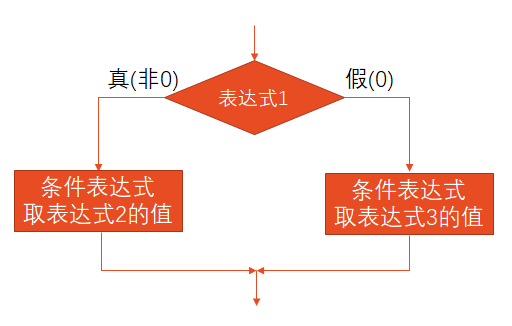
\includegraphics[scale=0.3]{if3}
\end{columns}
\end{frame}

\begin{frame}[shrink,fragile]{例: 大写转小写字母}
[例4.4, p96]输入一个字符, 判别它是否为大写字母, 如果是,将它转换成小写字母; 如果不是, 不转换。然后输出最后得到的字符。
\begin{lstlisting}
char ch;
scanf("%c",&ch);
ch = (ch>='A' && ch<='Z') ? (ch+32) : ch;
// 等效于
if(ch>='A' && ch<='Z')
{
   ch = ch+32; // 可简写为 ch += 32;
}
printf("ch=%c\n",ch);
\end{lstlisting}
\end{frame}

\section{数学表达式与C语言表达式的不同}

\begin{frame}[shrink,fragile]{数学表达式与C语言表达式的不同}
\begin{lstlisting}
int a = 100;
if(20 <= a && a <= 30) // 表达式的值为假(0), 条件表达式与数学含义相同
{ ...  }
if(20 <= a <= 30) // (20<=a)<=30, 表达式为真(1), 条件表达式与数学含义不同
{ ...  }
// 类似的
// if(a==20) 与 if(a=20)意义不同
if(a==20) //表达式的值是假(0), a的值没有变化
{ ... }
if(a=20) //表达式的值是10, 非0, 表示为真, 并且a被赋值为20(赋值语句)
{
    printf("%d\n",a); // 20 
}
printf("%d\n",a); // 20 
\end{lstlisting}
\end{frame}

\note{课堂讲解三角形判断, 掌握: \lstinline|&&,||,!|}

\section{用switch语句实现多分支选择结构}

\begin{frame}[shrink,fragile]{用switch语句实现多分支选择结构}
switch(int或char型表达式)
\begin{columns}[T]
\column{0.3\textwidth}
\begin{lstlisting}
int a;
scanf("%d",&a)
switch(a)
{
   case 10: 多条语句1; 
            break;
   case 20: 多条语句2; 
            break;
   case 30: 多条语句3; 
            break;
   default: 多条语句4;
}
\end{lstlisting}
\column{0.2\textwidth}
\vspace{3cm}
$\implies$
\column{0.3\textwidth}
\begin{lstlisting}
int a;
scanf("%d",&a)
if(a == 10)
{ 多条语句1; } 
else if(a == 20 )
{ 多条语句2; } 
else if(a == 30) 
{ 多条语句3; }
else
{ 多条语句4; }
\end{lstlisting}
\end{columns}
\end{frame}

\begin{frame}[shrink,fragile]
\begin{columns}[T]
\column{0.5\textwidth}
\begin{lstlisting}
char a; // 或 int a;
scanf("%c",&a)
swach(a)
{
    case 'A':
    case 'a': 多条语句1; 
              break;
    case 'B':
    case 'b': 多条语句2; 
              break;
    case 'C':
    case 'c': 多条语句3; 
              break;
    default: 多条语句4;
}
\end{lstlisting}
\column{0.5\textwidth}
\begin{lstlisting}	
char a; // 或 int a;
scanf("%d",&a)
if(a == 'A' || a == 'a')
{ 多条语句1; } 
else if(a == 'B' || a == 'b')
{ 多条语句2; } 
else if(a == 'C' || a == 'c') 
{ 多条语句3; }
else
{ 多条语句4; }
\end{lstlisting}
\end{columns}
\end{frame}

\begin{frame}[shrink,fragile]
\begin{columns}[T]
\column{0.4\textwidth}
\small
[例4.10,p99]运输公司对用户计算运输费用。路程越远,运费越低。标准如下:  
\begin{align*}
s<250 &&\text{没有折扣}\\
250\le s < 500 &&\text{2\%折扣}\\
500\le s < 1000 &&\text{5\%折扣}\\
1000\le s < 2000 &&\text{8\%折扣}\\
2000\le s < 3000 &&\text{10\%折扣}\\
3000\le s  &&\text{15\%折扣}
\end{align*}
\column{0.6\textwidth}
\vspace{-0.4cm}
\begin{lstlisting}
int c,s; //c是分类整数, s是距离
float p,w,d,f; //单价,重量,折扣,运费
// 运费 f = p*w*s*(1-d%) 
scanf("%f%f%d",&p,&w,&s);
if(s>=3000) { c = 12; } else {c = s/250; }
switch(c) {
   case 0: d=0; break;
   case 1: d=2; break;
   case 2: case 3: d=5; break;
   case 4: case 5: case 6: case 7: 
        d=8; break;
   case 8: case 9: case 10: case 11: 
        d=10 break;
   case 12: d=15; break;
}
f = p*w*s*(1-d/100);  printf("%.2f\n",f);
\end{lstlisting}
\end{columns}
\end{frame}
